\documentclass[12pt,a4paper]{article}
%\usepackage{ctex}
\usepackage{amsmath,amscd,amsbsy,amssymb,latexsym,url,bm,amsthm}
\usepackage{epsfig,graphicx,subfigure}
\usepackage{enumitem,balance}
\usepackage{wrapfig}
\usepackage{mathrsfs,euscript}
\usepackage[usenames]{xcolor}
\usepackage{tikz}
\usepackage{tikz-qtree}
\usepackage{hyperref}
\usepackage[vlined,ruled,linesnumbered]{algorithm2e}
\hypersetup{colorlinks=true,linkcolor=black}

\newtheorem{theorem}{Theorem}
\newtheorem{lemma}[theorem]{Lemma}
\newtheorem{proposition}[theorem]{Proposition}
\newtheorem{corollary}[theorem]{Corollary}
\newtheorem{exercise}{Exercise}
\newtheorem*{solution}{Solution}
\newtheorem{definition}{Definition}
\theoremstyle{definition}

\renewcommand{\thefootnote}{\fnsymbol{footnote}}

\newcommand{\postscript}[2]
 {\setlength{\epsfxsize}{#2\hsize}
  \centerline{\epsfbox{#1}}}

\renewcommand{\baselinestretch}{1.0}

\setlength{\oddsidemargin}{-0.365in}
\setlength{\evensidemargin}{-0.365in}
\setlength{\topmargin}{-0.3in}
\setlength{\headheight}{0in}
\setlength{\headsep}{0in}
\setlength{\textheight}{10.1in}
\setlength{\textwidth}{7in}
\makeatletter \renewenvironment{proof}[1][Proof] {\par\pushQED{\qed}\normalfont\topsep6\p@\@plus6\p@\relax\trivlist\item[\hskip\labelsep\bfseries#1\@addpunct{.}]\ignorespaces}{\popQED\endtrivlist\@endpefalse} \makeatother
\makeatletter
\renewenvironment{solution}[1][Solution] {\par\pushQED{\qed}\normalfont\topsep6\p@\@plus6\p@\relax\trivlist\item[\hskip\labelsep\bfseries#1\@addpunct{.}]\ignorespaces}{\popQED\endtrivlist\@endpefalse} \makeatother

\begin{document}
\noindent

%========================================================================
\noindent\framebox[\linewidth]{\shortstack[c]{
\Large{\textbf{Lab02-Divide and Conquer}}\vspace{1mm}\\
CS214-Algorithm and Complexity, Xiaofeng Gao, Spring 2020.}}
\begin{center}
\footnotesize{\color{red}$*$ If there is any problem, please contact TA Yiming Liu.}

% Please write down your name, student id and email.
\footnotesize{\color{blue}$*$ Name:Zehao Wang  \quad Student ID:518021910976 \quad Email: davidwang200099@sjtu.edu.cn}
\end{center}

\begin{enumerate}
    \item
    \textbf{Quicksort} is based on the Divide-and-Conquer method. Here is the two-step divide-and-conquer process for sorting a typical subarray $A[p \ldots r]$:
    \begin{enumerate}

    	\item
    	\textbf{Divide:} Partition the array $A[p \ldots r]$ into two subarrays $A[p \ldots q-1]$ and $A[q+1 \ldots r]$ such that each element of $A[p \ldots q-1]$ is less than or equal to $A[q],$ which is, in turn, less than or equal to each element of $A[q+1 \ldots r].$ Compute the index $q$ as part of this partitioning procedure.
    	
    	\item
    	\textbf{Conquer:} Sort $A[p \ldots q-1]$ and $A[q+1 \ldots r]$ respectively by recursive calls to Quicksort.
    	
    \end{enumerate}
    Write down the recurrence function $T(n)$ of QuickSort and compute its time complexity.

    {\color{purple}Hint: At this time $T(n)$ is split into two subarrays with different sizes (usually), and you need to describe its recurrence relation by the sum of two subfunctions plus additional operations.}
    \begin{solution}
    	\textbf{QuickSort} first requires randomly selecting a pivot and rearrange the array into two parts:one smaller than pivot and the other smaller than the pivot.This step requires $(n-1)$ comparisons and swaps.
    	
    	Then recursively sort the two parts.
    	
    	Assumes that the pivot is randomly selected.Then every element in the array is equally possible to be selected as the pivot in the first call of \textbf{QuickSort} and the probability is $\frac{1}{n}$.
    	
    	Then the time complexity of \textbf{Conquer} is $\frac{1}{n}\sum_{i=1}^{n}(T(i-1)+T(n-i))=\frac{1}{n}\sum_{i=0}^{n-1}(T(i)+T(n-i-1))=\frac{2}{n}\sum_{i=0}^{n-1}T(i)$.
    	
    	Let $S(n)=\sum_{i=0}^{n-1}(T(i))$.Then the recursion function is:
    	\begin{equation}\label{E1}
    	    T(n)=(n-1)+\frac{2}{n}S(n-1)
    	\end{equation}
    	left-hand side and right-hand side both multiplied by $n$, we have :
    	\begin{equation}\label{E2}
    	    nT(n)=n(n-1)+2S(n-1)
    	\end{equation}
    	And we have 
    	\begin{equation}\label{E3}
    	    (n-1)T(n-1)=(n-1)(n-2)+2S(n-2)
    	\end{equation}
    	Equation \eqref{E2} minus Equation \eqref{E3}:
    	\begin{equation}
    	    nT(n)-(n-1)T(n-1)=2(n-1)+2T(n-1)
    	\end{equation}
    	left and right both divided by $n(n+1)$:
    	\begin{equation}
    	    \frac{T(n)}{n+1}-\frac{T(n-1)}{n}=\frac{2(n-1)}{n(n+1)}\approx\frac{2}{n}
    	\end{equation}
    	Therefore $\frac{T(n)}{n+1}\approx2\sum_{i=1}^{n}\frac{1}{n}$
    	
    	Therefore $T(n)\approx(n+1)\log(n)=O(nlogn)$.
    \end{solution}
    \item
    \textbf{MergeCount}. Given an integer array $A[1 \ldots n]$ and two integer thresholds $t_l \le t_u$, Lucien designed an algorithm using divide-and-conquer method (As shown in Alg.~\ref{Alg-MergeCount}) to count the number of ranges $(i,j)$ ($1 \leq i \leq j \leq n$) satisfying
    \begin{equation}\label{Eqn-MergeCount}
    t_l \leq \sum_{k=i}^{j}{A[k]} \leq t_u.
    \end{equation}

    Before computation, he firstly constructed $S[0 \ldots n+1]$, where $S[i]$ denotes the sum of the first $i$ elements of $A[1 \ldots n]$. Initially, set $S[0]=S[n+1]=0$, $low=0$, $high=n+1$.

\begin{minipage}[t]{0.90\textwidth}
	\begin{algorithm}[H]
		%\algsetup{footnotesize}
		%\scriptsize
		\KwIn{$S[0,\cdots,n+1]$, $t_l$, $t_u$, $low$, $high$.}
		\KwOut{$count$ = number of ranges satisfying Eqn.~\eqref{Eqn-MergeCount}.}
		\BlankLine
		\caption{MergeCount($S$, $t_l$, $t_u$, $low$, $high$)}
		\label{Alg-MergeCount}
		
		$count \leftarrow 0$; $mid\leftarrow \lfloor \frac{low+high}{2} \rfloor$\;
		
		\lIf{$mid=low$}{
			\Return{$0$}
		}
		
		$count\leftarrow MergeCount(S, t_l, t_u, low, mid)+ MergeCount(S, t_l, t_u, mid, high)$\;
		
		\For{$i = low$ \textbf{to} $mid-1$}{
			$m \leftarrow \left \{ \begin{array}{ll}
            \min\{m \mid S[m]-S[i] \ge t_l, m \in [mid, high-1]\}, & \text{if exists}\\
            high, & \text{if not exist}
            \end{array}\right.$\;
			
			$n \leftarrow \left \{ \begin{array}{ll}
            \min\{n \mid S[n]-S[i] > t_u, n \in [mid, high-1]\}, & \text{if exists}\\
            high, & \text{if not exist}
            \end{array}\right.$
			\tcp*[r]{\color{blue}BinarySearch is used to find $m$, $n$}
			$count \leftarrow count+n-m$\;
		}
		$Merge(S,low,mid-1,high-1)$  \tcp*[r]{\color{blue}Merge is used for two sorted arrays}
		
		\Return{$count$}\;
		
	\end{algorithm}
\end{minipage}

    {\color{purple}\textbf{Example:} Given $A = [1,-1,2]$, $lower = 1$, $upper = 2$, return 4. The resulting four ranges should be $(1,1)$, $(1,3)$, $(2,3)$, and $(3,3)$.}

    Is Lucien's algorithm correct? Explain his idea and make correction if needed. Besides, compute the running time of Alg.~\ref{Alg-MergeCount} (or the corrected version) by recurrence relation. {\color{blue}(Note: we can't implement Master's Theorem in this case. Refer Reference06 for more details.)}
    \begin{solution}
    	Lucien's idea is to solve the problem by Divide-and-conquer.
    	
    	First find such kind of $(i,j)$ such that All the elements are in the first half of the array.Then find such kind of $(i,j)$ such that All the elements are in the second half of the array.Finally find $(i,j)$ such that some elements are in the first half, and the other are in the second half.
    	
    	All the value assignments have $O(1)$ complexity, which can be ignored in the top level.
    	
    	The two \textbf{MergeCount}'s with inputs of $\frac{n}{2}$ in size have complexity of $2T(\frac{n}{2})$.
    	
    	Line 5 and 6 have complexity of $O(nlogn)$ because \textbf{BinarySearch} has a complexity of $O(logn)$ and it is executed $n$ times on average.
    	
    	The \textbf{Merge} at last has a complexity of $O(n)$.
    	
    	Therefore the recursion function is $T(n)=2T(\frac{n}{2})+O(nlogn)$. \\
    	
    	\begin{figure}[htbp]
    		\centering
    		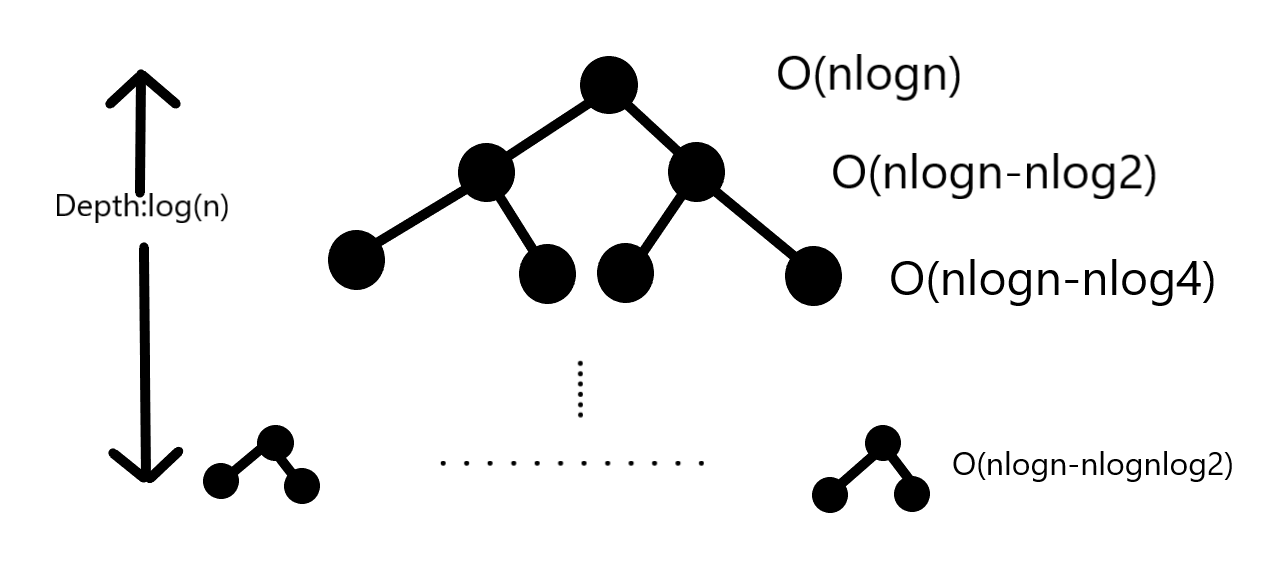
\includegraphics[width=0.8\textwidth]{test.png}
    		\caption{Reccurrence Tree}\label{Recurrence}
    	\end{figure}
    
    	Let $n=2^k$.Then $k=logn$.From the recursion tree we can get
    	
    	 $T(n)=n\log n+2\times(\frac{n}{2}\log(\frac{n}{2}))+4\times(\frac{n}{4}\log(\frac{n}{4}))+\cdots$
    	
    	$=k2^k+2(k-1)\times2^{k-1}+\cdots$
    	
    	$=k2^k+(k-1)2^k+\cdots+1\times2^k$
    	
    	$=2^k\times\frac{k(k+1)}{2}$
    	
    	$=n\frac{\log n(\log n+1)}{2}$
    	
    	$=O(n\log^2n)$
    \end{solution}
    \item
    \textbf{Batcher's odd-even merging network.} In this problem, we shall construct an \textbf{\textit{odd-even merging network}}. We assume that $n$ is an exact power of $2$, and we wish to merge the sorted sequence of elements on lines $\left\langle a_{1}, a_{2}, \ldots, a_{n}\right\rangle$ with those on lines $\left\langle a_{n+1}, a_{n+2}, \ldots, a_{2n}\right\rangle .$ If $n=1$, we put a comparator between lines $a_{1}$ and $a_{2}$. Otherwise, we recursively construct two odd-even merging networks that operate in parallel. The first merges the sequence on lines $\left\langle a_{1}, a_{3}, \ldots, a_{n-1}\right\rangle$ with the sequence on lines $\left\langle a_{n+1}, a_{n+3}, \ldots, a_{2n-1}\right\rangle$ (the
    odd elements). The second merges $\left\langle a_{2}, a_{4}, \ldots, a_{n}\right\rangle$ with $\left\langle a_{n+2}, a_{n+4}, \ldots\right.$
    $\left.a_{2n}\right\rangle$ (the even elements). To combine the two sorted subsequences, we put a comparator between $a_{2i}$ and $a_{2i+1}$ for $i=1,2, \ldots, n-1$.
    \begin{enumerate}
    	\item Replace the original Merger (taught in class) with Batcher's new Merger, and draw $2n$-input sorting networks for $n=8, 16, 32, 64$. {\color{blue}(Note: you are not forced to use Python Tkinter. Any visualization tool is welcome for this question.)}	
    	
    		\begin{figure}[htbp]
    			\centering
    			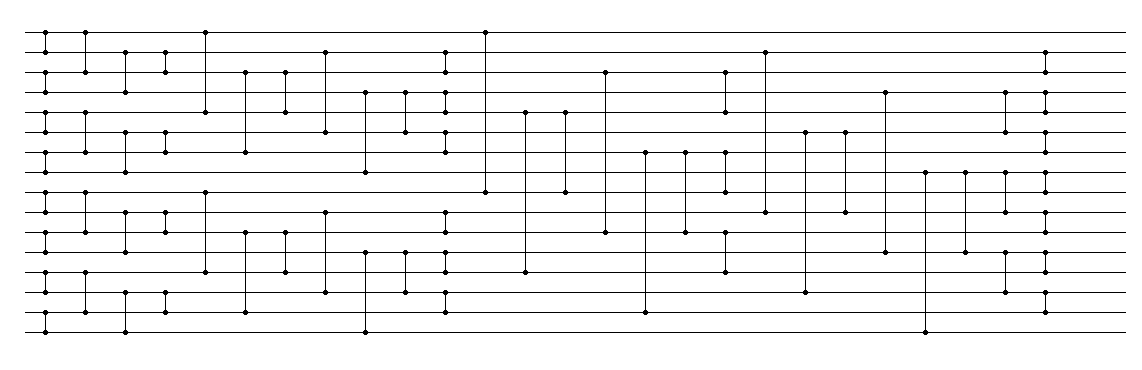
\includegraphics[width=0.8\textwidth]{n8.png}
    			\caption{n=8}\label{n8}
    		\end{figure}
    	    
    	    \begin{figure}[htbp]
    	    	\centering
    	    	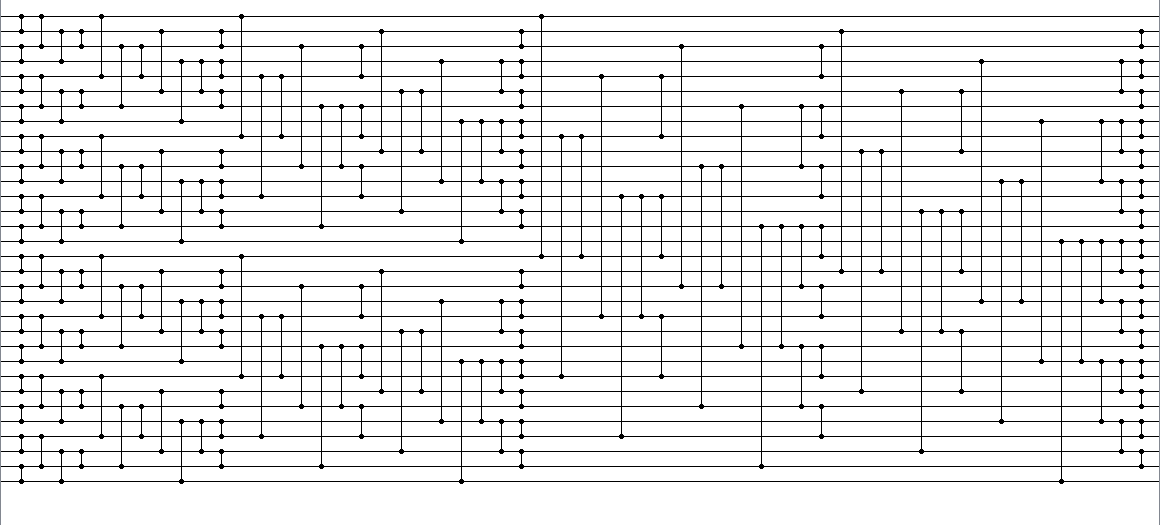
\includegraphics[width=0.8\textwidth]{n16.png}
    	    	\caption{n=16}\label{n16}
    	    \end{figure}
    	    \begin{figure}[htbp]
    	    		\centering
    	    		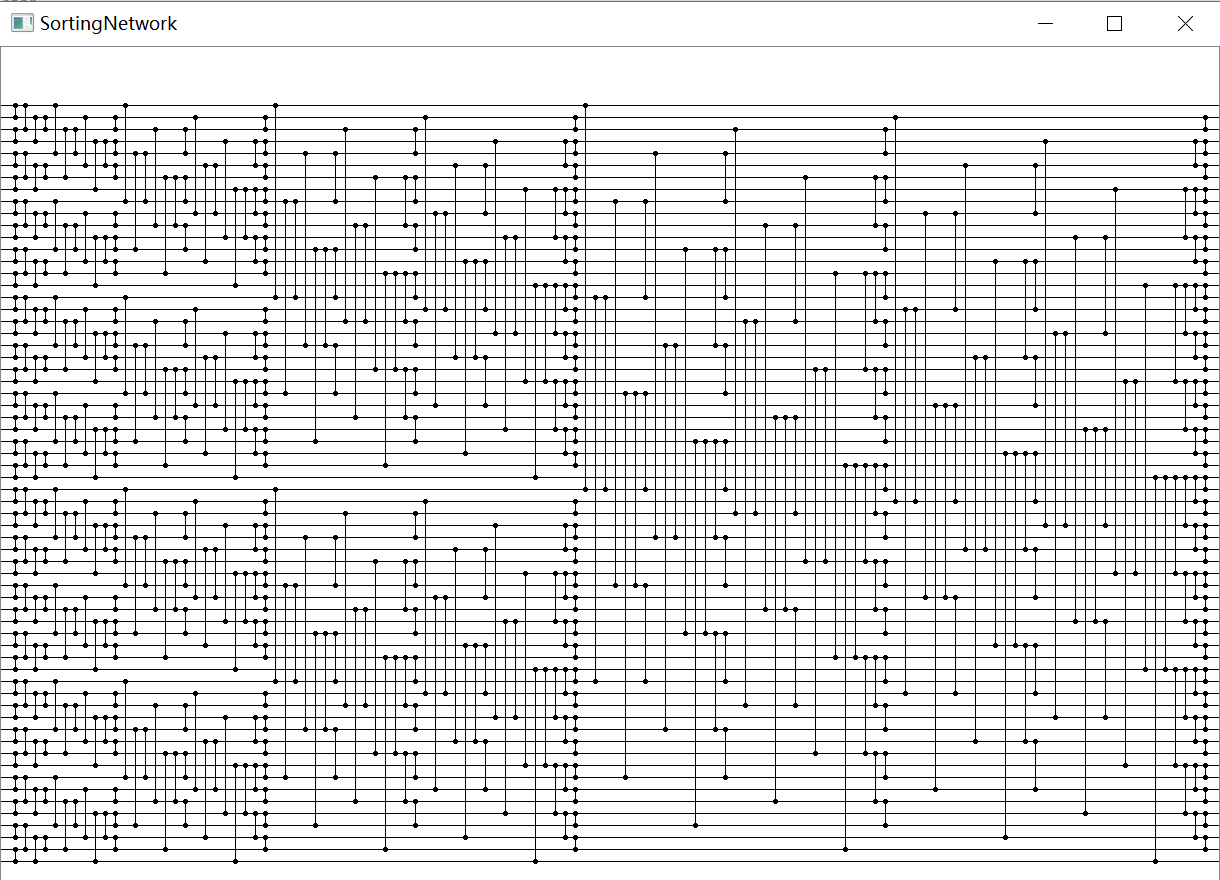
\includegraphics[width=0.8\textwidth]{n32.png}
    	    		\caption{n=32}\label{n32}
    	    \end{figure}
        	\begin{figure}[htbp]
        		\centering
        		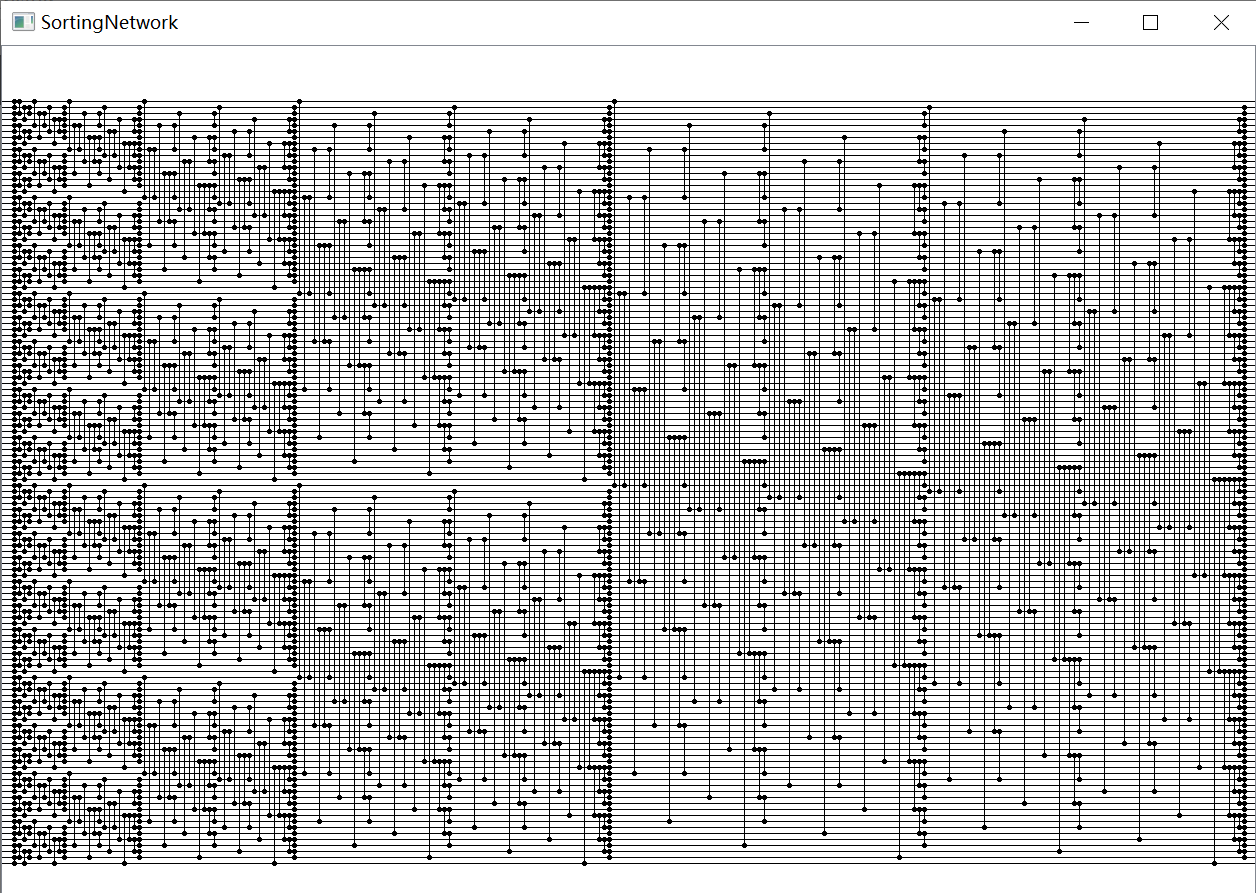
\includegraphics[width=0.8\textwidth]{n64.png}
        		\caption{n=64}\label{n64}
        	\end{figure}
        \quad\\
        \begin{solution}
        	The picture above is drawn with Qt.\\
        	"mainwindow.h","mainwindow.cpp""main.cpp""SortingNetwork.pro" are the source files.
        \end{solution}
    	
    	\item What is the depth of a $2n$-input odd-even sorting network?
    	    \begin{solution}
    	    	Assume that the depth of a $2n$-input odd-even sorting network is $D(n)$.
    	    	
    	    	An $2n$-input odd-even sorting network is made up of $2$ parallel $n$-input odd-even sortint network and a $2n$-input odd-even merging network.
    	    	
    	    	As for an $2n$-odd-even merging network, it is made up of comparators with the length of $n=2^k$,$\frac{n}{2}=2^{k-1}$,$\cdots$,$1=2^0$.
    	    	
    	    	Therefore it has a length of $\log n+1$.
    	    	
    	    	Therefore the recursion function of odd-even sorting network is:
    	    	
    	    	\begin{equation}
    	    	    \begin{cases}
    	    	    D(1)=1\\
    	    	    D(n)=D(\frac{n}{2})+\log n+1
    	    	    \end{cases}
    	        \end{equation}
    	    	
    	    	Therefore the depth of a $2n$-input odd-even sorting network is:
    	    	
    	    	 $\frac{\log^2 n}{2}+\frac{3\log n}{2}+1=O(\log^2 n)$.
    	    \end{solution}
    	\item
    	{\color{red}{(Optional Sub-question with Bonus)}} Use the zero-one principle to prove that any $2n$-input odd-even merging network is indeed a merging network.
    	\begin{proof}
    		Prove that $2n$-input odd-even merging network can work well on merging 0-1 arrays  by induction.
    		
    		\begin{itemize}
    			\item 
    			    When $n=1$, only one comparator is needed. Obviously a comparator can sort a 0-1 array with 2 elements in nondecreasing order.
    			    
    			\item 
    			    When $n=\frac{k}{2}$, assume that $k$-input merging network can sort the $k$-sized 0-1 arrays in nondecreaseing order.
    			\item 
    			    Then when $n=k$, to build a $2k$-input merging network, we need to merge two $k$-sized arrays and then use a combiner to combine the two subarrays.
    			\item    
    			    The two $k$-sized arrays can be sorted in nondecreasing order separately, according to the former assumption.
    			\item 
    			    In $\left\langle a_1,a_2,\ldots,a_k\right\rangle$, the number of $0$'s is either odd or even.And the ranks of $0$'s are all smaller than $1$'s.So it is with $\left\langle a_{k+1},a_{k+2},\ldots,a_{2k}\right\rangle$.
    			    
    			    Therefore there are at most 2 more $0$'s in $\left\langle a_1,a_3,\ldots,a_{2k-1}\right\rangle$ than in $\left\langle a_2,a_4,\ldots,a_{2k}\right\rangle$.This happens when the number of $0$'s in $\left\langle a_1,a_2,\ldots,a_k\right\rangle$ and $\left\langle a_{k+1},a_{k+2},\ldots,a_{2k}\right\rangle$ are both odd numbers.(For example,consider $\left\langle0,0,0,1,1,1,1,1,0,0,0,0,0,1,1,1\right\rangle$.)
    			\item    
    			    We have assumed that the two $k$-sized subarrays can be sorted in nondecreasing order separately,but in the case above,there is a $010$ subarray in $\left\langle a_1,a_2,\ldots,a_{2k}\right\rangle$,and the rank of the $1$ is an even number.(The example array above can be sorted into $\left\langle0,0,0,0,0,0,0,1,0,1,1,1,1,1,1,1\right\rangle$.)
    			    
    			    Then the $1$ can be swapped with the $0$ behind it with the help of combiner, which can make the array a completely sorted one.
    			    
    			\item 
    			    In other cases, the combiner is not neccessary because there is no such subarray like $010$.The array is sorted even without the combiner.
    			    
                \item 
                    Therefore the odd-even merger and the combiner can make sure $\left\langle a_1,a_2,\ldots,a_{2k}\right\rangle$ are sorted in nondecresing order.
    			    
    			\item 
    			    By 0-1 principle and induction, Batcher's odd-even merging network is really a merging network.
    			    
    			    
    		\end{itemize}
    	\end{proof}
    	
    \end{enumerate}

\end{enumerate}

\vspace{20pt}

\textbf{Remark:} You need to include your .pdf, .tex and .py files (or other possible sources) in your uploaded .rar or .zip file.

%========================================================================
\end{document}
